\documentclass[12pt]{article}
\usepackage{sbc-template}
\usepackage[utf8]{inputenc}
\usepackage[T1]{fontenc}
\usepackage[brazil]{babel}
\usepackage{amsmath,amssymb,graphicx,url,booktabs,longtable,array}
\title{Construção gulosa randomizada, VND e busca tabu para a localização de locais de prova}
\author{Bruno Keil\inst{1}}
\address{Departamento de Ciência da Computação -- Universidade Federal de Juiz de Fora\\DCC136 -- Inteligência Computacional -- 2026.3}
\begin{document}
\maketitle
\begin{abstract}
We implement and evaluate a randomized greedy constructor, variable neighborhood descent and tabu search for exam location and candidate assignment. Each school offers up to K exam types, with K=1 or K=2 selected at run time and type assignment chosen by the algorithm. An aggregate integer model certifies maximum attendance, while heuristics minimize travel distance. Experiments use 28 distinct instances, both K values and 30 seeds per method, totaling 3360 runs. Independent validation checks every initial and final assignment. We discuss design choices, initial and final variability, complete timing, a worked example and feasibility changes across K.
\end{abstract}
\begin{resumo}
Implementamos e avaliamos uma construção gulosa randomizada, descida em vizinhanças variáveis (VND) e busca tabu para selecionar locais de prova e alocar candidatos. Cada escola oferece até $K$ tipos de exame, com $K=1$ ou $K=2$ definido na execução e tipos escolhidos pelo algoritmo. Um modelo inteiro agregado certifica o atendimento máximo; as heurísticas minimizam a distância. Os experimentos usam 28 instâncias distintas, ambos os valores de $K$ e 30 sementes por método (3360 execuções), com validação independente de todas as alocações iniciais e finais. Apresentamos decisões de projeto, dispersão inicial/final, tempos completos, um exemplo passo a passo e o efeito de $K$ na viabilidade.
\end{resumo}

\section{Problema e objetivos}
O problema consiste em selecionar locais de prova e associar cada candidato a um único local compatível com seu tipo de exame, respeitando capacidades e minimizando a soma das distâncias. O contexto é o planejamento de exames de ingresso em universidades, conforme a referência indicada no enunciado~\cite{oliveira2021}. Uma solução de boa qualidade reduz o deslocamento agregado sem sacrificar o atendimento.

Consideramos as correções posteriores da professora: o limite de tipos por escola é um parâmetro de execução ($K=1$ ou $K=2$), e a escolha dos tipos permanece a cargo do algoritmo. Ambos os casos integram os experimentos. O endereço do repositório consta da Seção~\ref{sec:repro}.

Sejam $C$ os candidatos, $L$ as escolas, $T$ os tipos, $t_i$ o tipo do candidato $i$, $d_{ij}$ a distância da matriz e $Q_j$ a capacidade total das salas da escola $j$. Usamos capacidade agregada por escola: as salas fornecem capacidade e não são decisões independentes. Latitude/longitude não substituem a matriz. CEPs e identificadores são preservados; a ordem de linhas define os índices da matriz.

Com $a_i\in L$ e $S_j\subseteq T$, procuramos minimizar
\begin{equation}
 D(a)=\sum_{i\in C}d_{i,a_i},\quad
 |S_j|\leq K,\quad t_i\in S_{a_i},\quad
 \sum_i [a_i=j]\leq Q_j.
\end{equation}
A escola é utilizada se recebe pelo menos um candidato. Não há custos de abertura no objetivo, nem limite adicional para o número de escolas utilizadas.

\section{Representação e certificação de atendimento}
A solução contém um vetor $a$ de escolas, máscaras de bits $S_j$ para os tipos habilitados, cargas totais e por tipo, distância, excesso de capacidade e contagens de candidatos não alocados e incompatíveis. O valor $a_i=-1$ identifica explicitamente um candidato não atendido. Distâncias com até seis casas decimais são armazenadas como inteiros de milionésimos de km, evitando erros acumulados de ponto flutuante.

A soma das capacidades ser maior que o número de candidatos não garante atendimento completo: o limite de $K$ tipos pode impedir uma distribuição compatível. A condição $|T_+|\leq K|L|$, em que $T_+$ contém os tipos com demanda positiva, é necessária, mas não suficiente. Antes da heurística, resolvemos o seguinte modelo agregado, com $b_t$ candidatos de tipo $t$, $z_{jt}$ binária (tipo $t$ habilitado na escola $j$) e $x_{jt}\geq 0$ (candidatos de tipo $t$ atendidos em $j$):
\begin{align}
\max\;&\sum_{j,t}x_{jt} \\
\text{s.a. }&\sum_jx_{jt}\leq b_t &&\forall t,\\
&\sum_tx_{jt}\leq Q_j &&\forall j,\\
&x_{jt}\leq Q_jz_{jt},\quad \sum_tz_{jt}\leq K &&\forall j,t.
\end{align}
Somente $z$ é declarada inteira no solver: fixado $z$, o problema em $x$ é de transporte, com matriz totalmente unimodular e dados inteiros, e portanto admite ótimo inteiro; a implementação arredonda $x$ e verifica capacidade, demanda, limite $K$ e valor objetivo antes de aceitar o certificado. O ótimo $C^*$ certifica o atendimento máximo. Como não há restrições individuais além do tipo, uma solução inteira dessas contagens corresponde a uma alocação de candidatos. SciPy/HiGHS é uma dependência explícita dessa pré-checagem~\cite{scipy}. O solver não otimiza distâncias. Seu limite de 120 segundos, se atingido sem prova, produz erro inconclusivo, nunca uma declaração de inviabilidade.

Para escolas com tipos fixos, calculamos o atendimento por fluxo máximo: fonte--tipos com capacidade $b_t$, tipos--escolas compatíveis e escolas--sorvedouro com capacidade $Q_j$. Se $C^*<|C|$, o problema original é inviável. Nesse caso, a saída é marcada como tal e fornece uma solução parcial com exatamente $|C|-C^*$ não alocados. Primeiro maximizamos o atendimento e só então comparamos distâncias. Distâncias parciais não são comparáveis às de soluções completas.

\section{Construção da solução inicial}
\subsection{Escolha dos tipos e locais}
Começamos sem tipos habilitados. Para cada adição admissível $(j,t)$, calculamos o aumento $g_{jt}$ no atendimento por fluxo. Definimos $q_{jt}=\min(Q_j,b_t)$ e $h_{jt}$ como a média das $q_{jt}$ menores distâncias dos candidatos de tipo $t$ à escola $j$, normalizada por $\max(1,d_{\max})$ nas unidades inteiras. O critério é maximizar
\begin{equation}
 \mathrm{score}(j,t)=g_{jt}/b_t+g_{jt}/Q_j-h_{jt}.
\end{equation}
Os termos valorizam cobertura da demanda, aproveitamento de capacidade e proximidade. Consideramos somente ganhos positivos e escolas com menos de $K$ tipos. A lista restrita de candidatos (RCL) admite scores a partir de $s_{\max}-\alpha(s_{\max}-s_{\min})$. Com $\alpha=0$, a escolha é gulosa, com desempate por ordem de escola/tipo; com $\alpha>0$, sorteamos uniformemente na RCL.

Repetimos até alcançar $C^*$ ou estagnar. Uma escolha atrativa pode ocupar uma escola necessária para outro tipo. Para reparar esse impasse, exploramos adições, substituições e permutas de tipos, maximizando primeiro o fluxo e, em empate, reduzindo a soma das proximidades $h_{jt}$. Usamos primeira melhoria, até 20000 avaliações e no máximo 30 perturbações em platôs por tentativa. São até quatro tentativas para $\alpha>0$ e uma para $\alpha=0$. Se ainda não alcançarmos $C^*$, usamos os tipos certificados pelo modelo inteiro. Esse recurso é registrado como fallback; portanto, não se trata de um construtivo puramente independente do solver.

\subsection{Alocação por arrependimento e reparação}
Com os tipos definidos, cada candidato considera as escolas compatíveis com vaga. Seu arrependimento é a diferença entre a segunda e a primeira menor distância. Uma única opção tem prioridade infinita. Selecionamos por RCL de maior arrependimento e alocamos na escola disponível mais próxima. Candidatos com prioridade infinita são sorteados apenas entre si. Em $\alpha=0$, empates seguem a ordem do arquivo.

Quando uma escola lota, recalculamos as opções afetadas. Candidatos sem vaga compatível são tratados por caminhos aumentantes, encontrados em largura: candidato--escola cheia--candidato deslocado--outra escola--vaga. Aplicamos o caminho do final para o início. Cada cadeia aumenta o atendimento em uma unidade. Sem caminho aumentante, o atendimento é máximo para esses tipos; a fase anterior garante que esse máximo é $C^*$. Assim, em instâncias viáveis a construção produz uma solução completa; nas estruturalmente inviáveis, produz o melhor atendimento certificado.

\section{Avaliação, vizinhanças e estratégias de busca}
A avaliação usada na busca é
\begin{equation}
 f(s)=D(s)+\lambda E(s)+\mu\bigl(U(s)+I(s)\bigr),
\end{equation}
com $E$ igual ao excesso agregado, $U$ ao número de não alocados e $I$ ao de incompatíveis. Inicialmente $\lambda=\mu=|C|d_{\max}+1$ km; uma unidade de violação domina qualquer variação possível da distância. Compatibilidade e limite de tipos são invariantes das vizinhanças. A tabu pode explorar excesso temporário e destino $-1$; o arquivo de melhores soluções exige excesso e incompatibilidade nulos, prioriza menor $U$ e depois menor $D$.

Após cinco estados completos viáveis consecutivos, a tabu divide $\lambda$ por dois; após cinco inviáveis, dobra esse valor. O intervalo é de $\max(10^{-6}\text{ km},d_{\max}/10)$ a $16\lambda_0$; $\mu$ permanece fixo. Em casos estruturalmente inviáveis, $U>0$ impede uma sequência de viabilidade completa, o que é uma limitação dessa adaptação.

\textbf{N1: realocação.} Move um candidato para até $p$ escolas compatíveis mais próximas, excetuando a atual. Na tabu, também admite o destino $-1$. O delta de distância é $d_{ib}-d_{ia}$, com termos ausentes iguais a zero; distância e excesso são atualizados em tempo constante por movimento.

\textbf{N2: troca.} Permuta os destinos de dois candidatos do mesmo tipo, inclusive entre alocado e não alocado. O delta é $d_{ib}+d_{ha}-d_{ia}-d_{hb}$. A capacidade e o atendimento total não mudam. Selecionamos ganhos por par de escolas e tipo: o melhor candidato por arco no VND e os quatro melhores na tabu, permitindo alternativas a pares proibidos. Essa restrição limita a exploração da tabu.

\textbf{N3: alteração de tipos.} Adiciona ou substitui um tipo, ou permuta tipos entre duas escolas. O fluxo elimina propostas incapazes de manter $C^*$. A reconstrução libera candidatos das escolas alteradas e também os candidatos dos tipos recém-habilitados em qualquer escola. Estes últimos precisam ser reconsiderados para aproveitar uma escola antes vazia. Os demais candidatos são preservados; caminhos aumentantes podem deslocá-los. As propostas são embaralhadas, com orçamento de reconstruções por chamada.

\textbf{VND.} Usamos a ordem fixa $N_1, N_2, N_3$, das vizinhanças mais baratas e locais para a mais cara e estrutural. Uma \emph{iteração} do VND é uma exploração completa da vizinhança corrente $N_k$ com melhor melhoria: todos os movimentos examinados de $N_k$ são avaliados e o de menor $\Delta f$ é guardado. Se $\Delta f<0$, o movimento é aplicado e a busca volta a $N_1$ ($k\leftarrow 1$); caso contrário, passa para $N_{k+1}$. Assim, cada iteração aplica no máximo um movimento, e iterações sem melhora apenas avançam $k$. A busca termina quando $N_3$ também não melhora, isto é, no ótimo local simultâneo das três vizinhanças examinadas. Não há limite de iterações efetivo: o teto de $10^6$ existe apenas como salvaguarda contra laços e nunca foi atingido. A implementação também oferece primeira melhoria; a campanha usa melhor melhoria. As penalidades iniciais mantêm a viabilidade da descida a partir da construção.

\textbf{Busca tabu.} Examina N1/N2 a cada iteração e N3 a cada 20 iterações (e a cada 20 iterações sem melhora), escolhendo o menor delta admissível, inclusive positivo; cada iteração aplica exatamente um movimento. Os atributos tabu são candidato/escola deixada, par de candidatos e escola/tipo removido, com duração uniforme em $[5,12]$. A aspiração permite um movimento proibido se produzir a primeira solução completa viável ou melhorar a melhor completa viável conhecida. A tabu devolve a melhor solução arquivada, não necessariamente o último estado visitado. Ela para após 1000 iterações ou 200 iterações consecutivas sem melhorar a melhor solução.

Como N3 é amostrada, N1 usa lista restrita e N2 na tabu usa top-4, o ótimo local do VND refere-se às vizinhanças efetivamente examinadas; o encerramento não prova ótimo local das vizinhanças completas nem ótimo global.

\section{Exemplo passo a passo e caso de falha}
\label{sec:exemplo}
A instância didática \path{entrega/exemplo8_K1.txt} possui oito candidatos, dois tipos e escolas com capacidades 4, 4 e 2. Ela demonstra o caso $K=1$, com um tipo por escola; a formulação e o algoritmo também admitem $K=2$. A matriz é:
\begin{center}\begin{tabular}{ccrrr}
\toprule Candidato & Tipo & E1 & E2 & E3\\\midrule
C1&M1&8&10&6\\C2&M1&5&3&3\\C3&M1&14&11&1\\C4&M1&6&9&8\\
C5&M2&10&2&6\\C6&M2&9&10&12\\C7&M2&1&12&7\\C8&M2&3&12&8\\\bottomrule
\end{tabular}\end{center}
Com $\alpha=0$, o construtivo habilita E1/M2 (score 1,589286, cobertura 4) e E2/M1 (score 1,410714, cobertura 8). Como já atende todos, E3 fica sem tipo. C1--C4 vão a E2, e C5--C8 a E1. O custo é $(10+3+11+9)+(10+9+1+3)=56$ km.

N1 não tem outro destino compatível; N2 não muda escolas entre candidatos de mesmo tipo. N3 habilita M1 em E3 e reconstrói os candidatos M1. Os arrependimentos são 10 para C3, 4 para C1, 1 para C4 e 0 para C2. C3 e C1 ocupam E3; C2 e C4 permanecem em E2. O custo passa a $(1+6)+(3+9)+(10+9+1+3)=42$ km: $\Delta=-14$ km, redução de 25\%. Cargas finais: E1=4/4, E2=2/4, E3=2/2. Nenhuma escola recebe dois tipos.

Para facilitar a reprodução didática, usamos orçamento de 1000 reconstruções em N3, suficiente para todas as propostas desse exemplo. Esse orçamento difere das seis reconstruções da campanha. O trace literal está em \path{docs/exemplo8_K1-trace.txt}. O transporte exato com tipos finais fixos confirma 42 km para essa configuração, sem provar a melhor escolha global de tipos.

A instância I2 G2 tem 109 candidatos, seis tipos com demanda positiva e cinco escolas, com 121 vagas. Em $K=1$, ela não admite atendimento completo: o limite de cinco tipos habilitados impede acomodar os seis tipos demandados. Em $K=2$, a contagem deixa de impedir o atendimento, e o modelo agregado certifica uma alocação completa. Essa mudança é efeito da restrição, não uma melhora da heurística. Um caso real de qualidade insuficiente mesmo no ótimo local ocorre em I2 G8 ($K=2$) e em I2 G9 ($K=1$): em I2 G8 ($K=2$), o VND para após cerca de 99 iterações médias com distância entre 125,37 e 653,10 km (média 329,64 km), enquanto a busca tabu atinge média de 107,87 km; em I2 G9 ($K=1$), o VND converge para soluções completas entre 13752,79 e 21098,42 km (média 15068,86 km, contra 14053,55 km da tabu), conforme detalhado na Seção 7. Isso evidencia ótimos locais de tipos e motiva mecanismos que aceitem pioras temporárias e explorem mais propostas em N3.

\section{Qualidade dos dados e decisões de projeto}
Dos 31 arquivos de entrada, 28 representam instâncias distintas utilizáveis. Duas duplicatas exatas foram identificadas, e um arquivo contendo apenas um caminho externo foi excluído. Dois arquivos apresentavam os cabeçalhos na mesma linha; a preparação apenas os separou em cópias, sem alterar valores. A auditoria registra hashes e critérios de inclusão em \path{instances/auditoria_atual.csv}.

A reconstrução em N3 precisa considerar o efeito global de uma mudança de tipos: preservar candidatos de todas as escolas inalteradas impedia ocupar uma escola recém-habilitada. Por isso, liberamos também os candidatos dos tipos novos, independentemente da escola atual. O exemplo da Seção 5 ilustra essa decisão, protegida por uma regressão automatizada. As verificações incluem recomputação independente de deltas e alocações, além de execução com AddressSanitizer e UndefinedBehaviorSanitizer.

Escolhemos $\alpha=0{,}3$ para restringir o sorteio à faixa superior de 30\% dos scores e arrependimentos, preservando preferência gulosa e introduzindo diversidade entre sementes. A RCL é definida pelo intervalo de valores, não por 30\% dos elementos. Não houve ajuste sistemático desse parâmetro: as estatísticas iniciais e finais quantificam a variabilidade resultante.

A lista de $p=5$ destinos em N1 concentra avaliações nas escolas compatíveis mais próximas e limita o custo de enumeração em instâncias grandes. Se houver menos de cinco alternativas, todas são consideradas. Essa economia pode perder movimentos úteis para liberar vagas; N2 e N3 ampliam a exploração por decisões diferentes.

A duração tabu uniforme em $[5,12]$ evita retorno imediato por pelo menos cinco iterações e varia a duração da proibição para reduzir ciclos sincronizados. O intervalo é uma escolha operacional, sem alegação de calibração ótima. A aspiração permite superar a memória quando um movimento melhora a melhor solução completa viável.

O VND não recebe orçamento: por definição, ele é uma descida que termina no ótimo local, e qualquer teto inferior ao comprimento natural da trajetória mede apenas uma descida interrompida. Uma campanha preliminar com teto de 150 iterações para ambos os métodos evidenciou esse problema: 527 das 840 execuções do VND em $K=1$ foram interrompidas antes do ótimo local, e em I2 G9 a distância média final do VND caía de cerca de 18800 km para cerca de 14600 km quando a descida era levada até o fim. Aquela comparação favorecia artificialmente a tabu, que, ao examinar N3 periodicamente, alcançava a vizinhança estrutural mais cedo. Os resultados preliminares estão preservados em \path{resultados/historico_iter150/} apenas para registro.

Para a tabu, que por construção não para em ótimos locais, adotamos 1000 iterações ou 200 sem melhora. O teto fornece orçamento reprodutível, independente da oscilação do tempo em máquina compartilhada; 200 iterações correspondem a dez avaliações periódicas de N3 sem progresso e interrompem trajetórias estagnadas. Os métodos não recebem o mesmo número de avaliações nem o mesmo tempo; por isso, reportamos tempos junto às distâncias e não inferimos eficiência apenas pelas iterações.

As seis reconstruções por chamada de N3 limitam o trabalho da vizinhança mais cara, que altera tipos e refaz parte das alocações. O embaralhamento varia as propostas examinadas, ao custo de poder omitir uma melhoria. O exemplo didático usa orçamento maior para tornar o passo reproduzível; a campanha mantém seis, explicitando esse compromisso entre exploração e custo. Na tabu, a avaliação de N3 a cada 20 iterações intercala mudanças estruturais com ajustes mais baratos de N1/N2.

\section{Experimentos e resultados}
A campanha principal foi executada \textbf{após a correção da N3}, sobre 28 instâncias distintas, com VND e tabu e 30 sementes por método (1 a 30), para cada $K\in\{1,2\}$, totalizando 3360 execuções e 6720 soluções iniciais/finais verificadas independentemente. São 1680 execuções em cada valor de $K$. As demais configurações são iguais: $\alpha=0{,}3$, $p=5$, seis reconstruções por chamada de N3 e tenure $[5,12]$. O VND usa melhor melhoria e executa até o ótimo local; a tabu usa até 1000 iterações, 200 sem melhoria e N3 a cada 20 iterações. O limite temporal é desativado. Cada iteração do VND é uma exploração de vizinhança, e cada iteração da tabu aplica um movimento; os números de iterações dos dois métodos, portanto, não são comparáveis entre si.

Cada execução registra custo inicial/final, melhoria absoluta/percentual, tempo de leitura, pré-checagem, construção e busca, escolas utilizadas, cargas por tipo e ocupação. Calculamos média, mínimo, máximo e desvio padrão amostral das distâncias tanto iniciais quanto finais. As tabelas completas do Apêndice A incluem ambos os valores de $K$. Usamos a identificação uniforme I1 G$n$ ou I2 G$n$ para a primeira ou segunda instância do grupo $n$, independentemente da grafia do arquivo original. A melhoria percentual é calculada por execução e depois promediada. A comparação entre métodos usa o mesmo conjunto de instâncias e sementes; não implica trajetórias idênticas após a construção. Casos inviáveis são descritos com atendimento parcial ótimo, sem compará-los a soluções completas.

Em $K=1$, 24 das 28 instâncias admitem atendimento completo. A comparação de distância média entre métodos resulta em 27 vitórias da tabu, 0 do VND e 1 empate. O fallback foi usado em 0 das 1680 construções desse caso.

Em $K=2$, 28 das 28 instâncias admitem atendimento completo. A comparação de distância média entre métodos resulta em 28 vitórias da tabu, 0 do VND e 0 empates. O fallback foi usado em 0 das 1680 construções desse caso.

As quatro inviabilidades em $K=1$ são I1 G2, I2 G2, I2 G3 e I2 G5; essa classificação depende de $K$. Em I2 G2 (109 candidatos, seis tipos e cinco escolas), o atendimento certificado passa de 96 em $K=1$ para 109 em $K=2$. A distância parcial de $K=1$ não mede a mesma tarefa da distância completa de $K=2$; portanto, não calculamos melhoria percentual entre esses dois casos.

O VND foi executado até o ótimo local em todas as execuções: o teto de segurança de 1000000 iterações foi atingido 0 vezes; a trajetória média teve 863 iterações e a mais longa 7016. A tabu atingiu o teto de 1000 iterações em 776 das 1680 execuções; nas demais, parou após 200 iterações sem melhora. A melhoria média sobre a construção foi de 12,87\% no VND e 22,22\% na tabu, com tempo médio de busca de 0,519 s e 1,628 s por execução, respectivamente.

O pior desempenho relativo do VND ocorreu em I2 G8 com $K=2$: a distância média final (329,64 km, desvio padrão 112,58) ficou 209,60\% acima da melhor solução conhecida (106,47 km, mínimo entre as 60 execuções dos dois métodos), e a pior semente ficou 513,41\% acima. A tabu obteve média de 107,87 km na mesma instância.

Todas as 6720 soluções iniciais/finais respeitaram capacidade e compatibilidade e atingiram o atendimento certificado. As contagens de vitórias são descritivas e comparam os métodos somente dentro da mesma instância, do mesmo K e do mesmo atendimento; não estabelecem significância estatística.

A pré-checagem é executada uma vez por lote de 30 sementes, separadamente para cada método e K. A tabela de tempos inclui esse custo integral em P e o amortiza em Total: $T_{\mathrm{total}}=(T_{\mathrm{leitura}}+P)/30+T_{\text{construção}}+T_{\mathrm{busca}}$. O custo do lote é 30 vezes esse total médio; não se trata de medição isolada com CPU exclusiva.

Ambiente: macOS (arm64), Python 3.9.6, C++17 com Apple Clang e otimização \texttt{-O2}, NumPy 1.24.2 e SciPy 1.11.3. VND e tabu foram executados simultaneamente, com quatro processos cada (oito processos em oito núcleos); os tempos incluem competição por CPU. Os manifestos registram entradas, binário e parâmetros. O prefixo do hash do binário é \texttt{a4274b9a6a7ffae1}.

\begin{table}[ht]
\centering\small
\setlength{\tabcolsep}{3pt}
\caption{Comparação de K=1 e K=2, 30 sementes por linha; distâncias em km. Inicial e Final: média $\pm$ desvio padrão amostral. U é o déficit certificado. Tempos e extremos constam do Apêndice A.}
\begin{tabular}{lrlrrrr}
\toprule Instância & K & Método & U & Inicial (média) & Final (média) & Melhora (\%)\\\midrule
I1 G1 & 1 & VND & 0 & 30517,89 $\pm$ 1221,73 & 28433,20 $\pm$ 793,03 & 6,73 \\
I1 G1 & 1 & TABU & 0 & 30517,89 $\pm$ 1221,73 & 27683,28 $\pm$ 692,47 & 9,19 \\
I1 G1 & 2 & VND & 0 & 29826,65 $\pm$ 974,77 & 27042,78 $\pm$ 923,86 & 9,27 \\
I1 G1 & 2 & TABU & 0 & 29826,65 $\pm$ 974,77 & 24405,59 $\pm$ 272,54 & 18,09 \\
I1 G2 & 1 & VND & 16 & 764,05 $\pm$ 7,15 & 754,98 $\pm$ 3,76 & 1,18 \\
I1 G2 & 1 & TABU & 16 & 764,05 $\pm$ 7,15 & 753,32 $\pm$ 0,00 & 1,40 \\
I1 G2 & 2 & VND & 0 & 903,66 $\pm$ 9,47 & 889,32 $\pm$ 6,78 & 1,58 \\
I1 G2 & 2 & TABU & 0 & 903,66 $\pm$ 9,47 & 878,30 $\pm$ 3,21 & 2,80 \\
I2 G2 & 1 & VND & 13 & 936,19 $\pm$ 40,57 & 885,42 $\pm$ 0,00 & 5,25 \\
I2 G2 & 1 & TABU & 13 & 936,19 $\pm$ 40,57 & 885,42 $\pm$ 0,00 & 5,25 \\
I2 G2 & 2 & VND & 0 & 986,39 $\pm$ 42,63 & 914,67 $\pm$ 8,82 & 7,10 \\
I2 G2 & 2 & TABU & 0 & 986,39 $\pm$ 42,63 & 903,11 $\pm$ 0,84 & 8,28 \\
I2 G8 & 1 & VND & 0 & 356,47 $\pm$ 108,49 & 241,71 $\pm$ 94,27 & 27,60 \\
I2 G8 & 1 & TABU & 0 & 356,47 $\pm$ 108,49 & 117,23 $\pm$ 0,56 & 63,06 \\
I2 G8 & 2 & VND & 0 & 479,04 $\pm$ 157,98 & 329,64 $\pm$ 112,58 & 26,50 \\
I2 G8 & 2 & TABU & 0 & 479,04 $\pm$ 157,98 & 107,87 $\pm$ 1,84 & 74,82 \\
\bottomrule\end{tabular}
\end{table}
\begin{figure}[ht]\centering
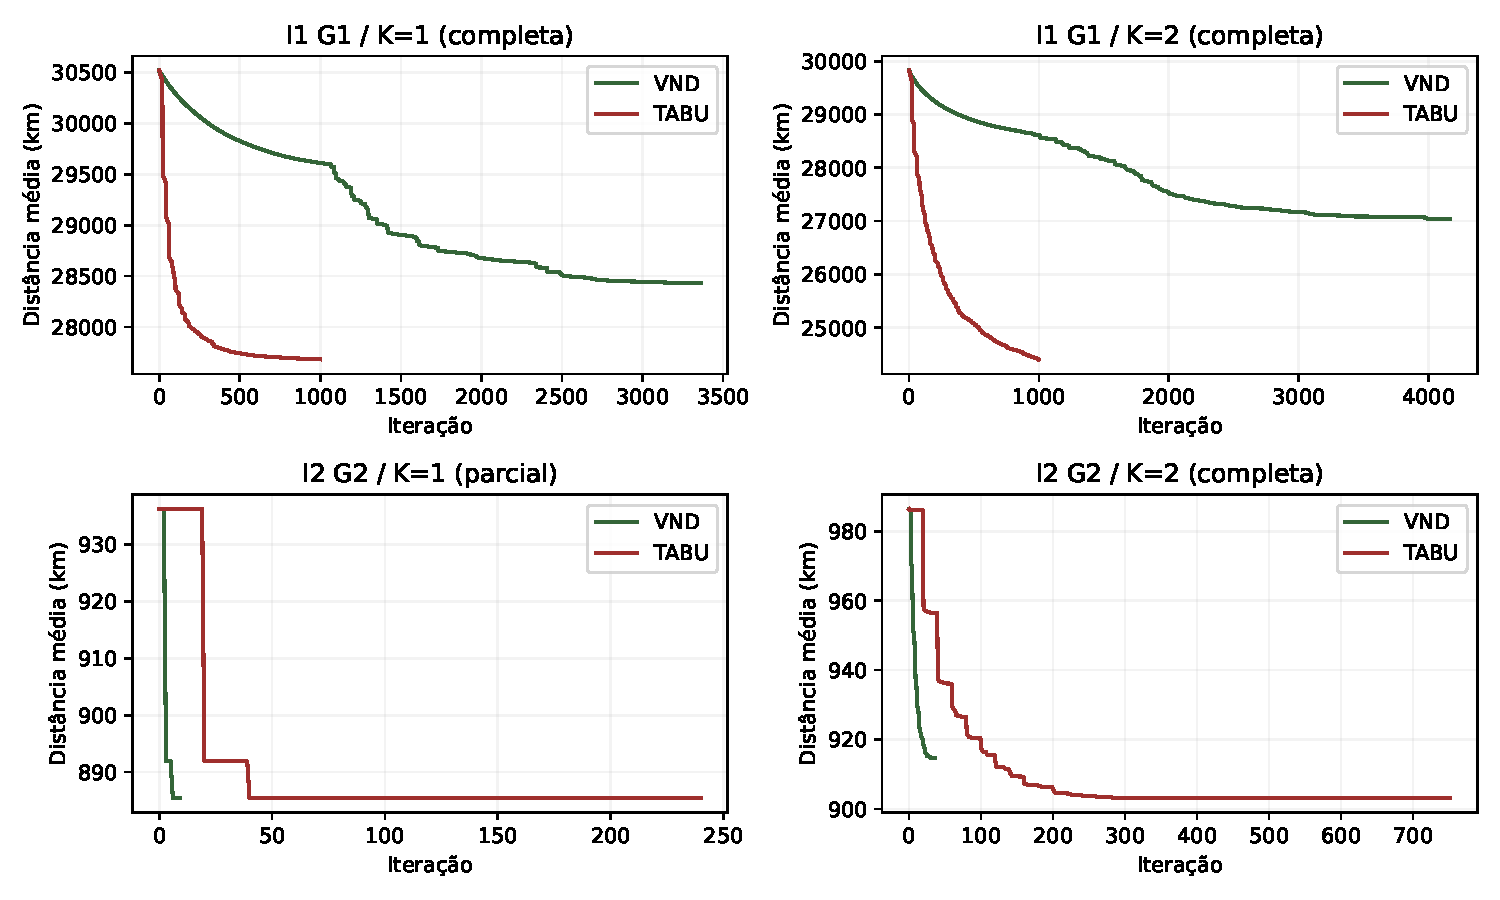
\includegraphics[width=\textwidth]{../resultados/final_convergencia.pdf}
\caption{Melhor distância média por iteração para instâncias selecionadas, em K=1 e K=2. As curvas parciais e completas de I2 G2 têm atendimentos diferentes e não medem a mesma tarefa. Curvas encerradas são mantidas no último valor; o eixo horizontal se estende até a execução mais longa de cada método, e as iterações de VND e tabu têm significados distintos. Distância parcial quando indicada no título.}
\end{figure}

O validador Python relê a instância e recompõe as distâncias com \texttt{Decimal}, sem reutilizar deltas do C++. Verifica IDs, capacidade, compatibilidade, atendimento certificado, ocupação e evolução da melhor solução. Os JSONs guardam cada atribuição e carga por escola/tipo. Os dados de $K=1$ estão em \path{resultados/final_vnd/} e \path{resultados/final_tabu/}. Para $K=2$, ficam em \path{resultados/final_k2_vnd/} e \path{resultados/final_k2_tabu/}. Os manifestos identificam entradas e configurações.

\section{Conclusões e limitações}
A combinação de escolha de tipos, arrependimento e caminhos aumentantes fornece soluções com o atendimento certificado. N1/N2 melhoram alocações com tipos fixos, enquanto N3 altera uma decisão estrutural que pode bloquear as primeiras vizinhanças. A auditoria do exemplo pequeno mostrou por que uma escola vazia precisa participar efetivamente da reconstrução, e não apenas receber um tipo na representação.

A abordagem depende de um solver inteiro para certificar atendimento e como salvaguarda da construção; nenhum fallback foi necessário nas 3360 construções observadas, o que não elimina essa dependência para novas entradas. A passagem de $K=1$ para $K=2$ permite atendimento completo nas quatro instâncias antes inviáveis, evidenciando a necessidade de analisar cada configuração separadamente. A busca de distância permanece heurística. Amostragem de N3, listas de candidatos e limites de iterações restringem a qualidade; tempos foram medidos em máquina compartilhada, com processos paralelos, sem isolamento de CPU. A análise é descritiva, sem testes de significância ou alegação de superioridade universal. Como continuidade, propomos ajustar a amostragem de N3, comparar orçamentos de tempo/avaliações, explorar mais trocas de tipos e melhorar a adaptação de penalidades nos casos de atendimento parcial.

\section{Reprodução e arquivos de entrega}
\label{sec:repro}
São necessários compilador C++17, Make e Python com NumPy e SciPy; Matplotlib é usado nas figuras. O repositório está em \url{https://github.com/brunokeil/Trabalho_Inteligencia_Computacional}. A apresentação tem versões HTML independente e PDF, com 12 slides e roteiro de dez minutos. O HTML contém os resultados e permite baixar o CSV e o relatório incorporados, mesmo quando movido para outra pasta; o link do GitHub requer internet. O código-fonte, instâncias, manifestos, resultados, relatório LaTeX/PDF e apresentação estão no pacote gerado por \path{scripts/empacotar.py}. Os comandos principais são:
\begin{verbatim}
make
make test
python3 scripts/preparar_instancias.py
sh scripts/campanha_final.sh   # 4 campanhas
python3 scripts/gerar_entrega.py
make report
\end{verbatim}
O script \path{scripts/campanha_final.sh} invoca \path{scripts/executar_todas.py} para VND (teto $10^6$) e tabu (teto 1000 e estagnação 200), com $K\in\{1,2\}$, 30 sementes e saídas \path{final_vnd}, \path{final_tabu}, \path{final_k2_vnd} e \path{final_k2_tabu} em \path{resultados/}.
Use outra pasta de saída quando o manifesto divergir. A mesma semente reproduz decisões no mesmo ambiente com limite de iterações; distribuições da biblioteca C++ e versões do solver podem alterar trajetórias entre plataformas. O README descreve a regeneração das tabelas, a exportação dos slides em PDF e o empacotamento da entrega.

\appendix
\section{Resultados completos e distribuição das soluções}
\small
\setlength{\tabcolsep}{3pt}
\begin{longtable}{llrrrrr}
\caption{Todas as instâncias: média, desvio padrão amostral, mínimo e máximo da distância; U é o déficit certificado.}\\
\toprule Instância & Método & U & Média & dp & Mínimo & Máximo\\\midrule\endfirsthead
\toprule Instância & Método & U & Média & dp & Mínimo & Máximo\\\midrule\endhead
I1 G1 & VND & 0 & 30204,54 & 1217,13 & 28072,65 & 33693,26 \\
I1 G1 & TABU & 0 & 28134,55 & 615,71 & 27189,80 & 29305,08 \\
I1 G10 & VND & 0 & 13108,63 & 1156,33 & 11328,14 & 15795,18 \\
I1 G10 & TABU & 0 & 11180,30 & 462,04 & 10606,33 & 12543,05 \\
I1 G11 & VND & 0 & 39179,98 & 3481,35 & 34967,38 & 46319,64 \\
I1 G11 & TABU & 0 & 35200,24 & 422,86 & 34967,19 & 37231,64 \\
I1 G12 & VND & 0 & 21278,90 & 1506,29 & 19656,01 & 25020,54 \\
I1 G12 & TABU & 0 & 20048,21 & 359,48 & 19300,21 & 20654,38 \\
I1 G2 & VND & 16 & 754,98 & 3,76 & 753,32 & 773,31 \\
I1 G2 & TABU & 16 & 753,44 & 0,40 & 753,32 & 755,47 \\
I1 G3 & VND & 0 & 1073,42 & 19,40 & 1042,94 & 1110,52 \\
I1 G3 & TABU & 0 & 1032,06 & 5,52 & 1026,20 & 1053,25 \\
I1 G4 & VND & 0 & 13293,90 & 873,21 & 12427,08 & 15573,34 \\
I1 G4 & TABU & 0 & 12566,70 & 125,24 & 12370,05 & 12809,68 \\
I1 G5 & VND & 0 & 16851,15 & 1253,16 & 14550,70 & 19124,60 \\
I1 G5 & TABU & 0 & 15110,67 & 322,90 & 14550,32 & 15742,77 \\
I1 G6 & VND & 0 & 19061,12 & 1352,03 & 16374,65 & 22518,87 \\
I1 G6 & TABU & 0 & 16718,26 & 276,26 & 16159,52 & 17322,38 \\
I1 G7(1) & VND & 0 & 23956,38 & 2568,16 & 21102,26 & 31465,82 \\
I1 G7(1) & TABU & 0 & 21620,32 & 678,42 & 20907,49 & 23722,12 \\
I1 G9 & VND & 0 & 11507,22 & 2595,73 & 7675,30 & 16539,78 \\
I1 G9 & TABU & 0 & 8246,65 & 695,48 & 7419,84 & 10005,24 \\
I2 G1 & VND & 0 & 17846,53 & 1398,47 & 15317,95 & 20451,39 \\
I2 G1 & TABU & 0 & 15368,47 & 482,14 & 14574,87 & 16560,06 \\
I2 G10 & VND & 0 & 14627,78 & 1101,56 & 12332,29 & 16715,63 \\
I2 G10 & TABU & 0 & 13518,62 & 608,00 & 12281,61 & 15147,50 \\
I2 G11 & VND & 0 & 105762,06 & 1603,20 & 103565,43 & 109787,34 \\
I2 G11 & TABU & 0 & 103042,56 & 226,10 & 102776,42 & 103708,26 \\
I2 G12 & VND & 0 & 97969,33 & 1277,37 & 95869,90 & 100716,08 \\
I2 G12 & TABU & 0 & 95562,25 & 644,64 & 94589,80 & 97390,21 \\
I2 G2 & VND & 13 & 885,42 & 0,00 & 885,42 & 885,42 \\
I2 G2 & TABU & 13 & 885,42 & 0,00 & 885,42 & 885,42 \\
I2 G3 & VND & 243 & 598,58 & 17,14 & 567,73 & 619,69 \\
I2 G3 & TABU & 243 & 524,73 & 1,74 & 520,81 & 528,54 \\
I2 G4 & VND & 0 & 12449,49 & 2304,08 & 9970,86 & 18441,75 \\
I2 G4 & TABU & 0 & 10391,34 & 659,16 & 9870,61 & 12604,96 \\
I2 G5 & VND & 20 & 16026,69 & 297,28 & 15409,24 & 16874,37 \\
I2 G5 & TABU & 20 & 14559,06 & 204,41 & 14383,96 & 15022,13 \\
I2 G6 & VND & 0 & 29298,96 & 896,34 & 27717,14 & 31327,96 \\
I2 G6 & TABU & 0 & 27745,19 & 210,82 & 27342,04 & 28150,71 \\
I2 G7 & VND & 0 & 70697,64 & 2007,08 & 66520,41 & 74196,48 \\
I2 G7 & TABU & 0 & 66470,08 & 1169,90 & 64862,86 & 69585,77 \\
I2 G9 & VND & 0 & 18768,47 & 3036,69 & 14281,20 & 24126,19 \\
I2 G9 & TABU & 0 & 14424,33 & 572,55 & 13699,57 & 15853,39 \\
I1 G8 & VND & 0 & 1273,18 & 38,26 & 1217,89 & 1349,71 \\
I1 G8 & TABU & 0 & 1232,86 & 20,26 & 1194,82 & 1278,43 \\
I2 G8 & VND & 0 & 241,71 & 94,27 & 119,31 & 453,80 \\
I2 G8 & TABU & 0 & 191,99 & 94,10 & 117,08 & 414,34 \\
I 1 G13 & VND & 0 & 1456,89 & 72,71 & 1319,68 & 1585,19 \\
I 1 G13 & TABU & 0 & 1399,02 & 50,09 & 1330,77 & 1528,79 \\
I 1 G14 & VND & 0 & 1465,28 & 35,80 & 1409,90 & 1566,82 \\
I 1 G14 & TABU & 0 & 1434,90 & 28,35 & 1391,32 & 1535,14 \\
I 2 G13 & VND & 0 & 1397,39 & 77,39 & 1311,85 & 1591,76 \\
I 2 G13 & TABU & 0 & 1355,23 & 50,60 & 1301,11 & 1502,74 \\
I 2 G14 & VND & 0 & 2139,70 & 139,27 & 1956,45 & 2444,53 \\
I 2 G14 & TABU & 0 & 2060,33 & 82,44 & 1956,45 & 2210,52 \\
\bottomrule\end{longtable}
\begin{longtable}{llrrrr}
\caption{Tempos médios por execução (segundos), locais usados e melhoria percentual média. C: construção; BL: busca. Pré-checagem fica nos CSVs e é compartilhada pelo lote.}\\
\toprule Instância & Método & C (s) & BL (s) & Locais & Melhora (\%)\\\midrule\endfirsthead
\toprule Instância & Método & C (s) & BL (s) & Locais & Melhora (\%)\\\midrule\endhead
I1 G1 & VND & 0,0691 & 0,1897 & 15,00 & 1,03 \\
I1 G1 & TABU & 0,0829 & 1,2840 & 15,00 & 7,72 \\
I1 G10 & VND & 0,0928 & 0,1478 & 15,00 & 2,17 \\
I1 G10 & TABU & 0,1248 & 0,8215 & 15,00 & 16,16 \\
I1 G11 & VND & 0,0378 & 0,1179 & 10,00 & 2,86 \\
I1 G11 & TABU & 0,0689 & 0,7105 & 10,00 & 12,24 \\
I1 G12 & VND & 0,0665 & 0,1925 & 15,00 & 5,97 \\
I1 G12 & TABU & 0,0720 & 0,6661 & 15,00 & 11,22 \\
I1 G2 & VND & 0,0003 & 0,0003 & 5,00 & 1,18 \\
I1 G2 & TABU & 0,0002 & 0,0016 & 5,00 & 1,38 \\
I1 G3 & VND & 0,1950 & 0,2431 & 20,00 & 0,18 \\
I1 G3 & TABU & 0,1603 & 1,0998 & 20,00 & 4,00 \\
I1 G4 & VND & 0,0680 & 0,1655 & 12,00 & 7,09 \\
I1 G4 & TABU & 0,0705 & 0,5564 & 12,00 & 12,09 \\
I1 G5 & VND & 0,0775 & 0,1491 & 15,00 & 2,66 \\
I1 G5 & TABU & 0,0814 & 0,6354 & 15,00 & 12,44 \\
I1 G6 & VND & 0,1379 & 0,1517 & 15,00 & 1,54 \\
I1 G6 & TABU & 0,0946 & 0,7061 & 15,00 & 13,32 \\
I1 G7(1) & VND & 0,0555 & 0,1420 & 11,00 & 8,80 \\
I1 G7(1) & TABU & 0,0473 & 0,3483 & 11,00 & 17,34 \\
I1 G9 & VND & 0,0679 & 0,1570 & 14,00 & 2,61 \\
I1 G9 & TABU & 0,0419 & 0,4542 & 14,00 & 27,66 \\
I2 G1 & VND & 0,1016 & 0,2238 & 14,90 & 1,30 \\
I2 G1 & TABU & 0,0633 & 0,8264 & 15,00 & 14,60 \\
I2 G10 & VND & 0,1291 & 0,1514 & 15,00 & 0,92 \\
I2 G10 & TABU & 0,0898 & 0,5972 & 15,00 & 8,03 \\
I2 G11 & VND & 0,1000 & 0,1449 & 14,90 & 0,22 \\
I2 G11 & TABU & 0,0585 & 0,5290 & 14,90 & 2,76 \\
I2 G12 & VND & 0,0741 & 0,1414 & 15,00 & 0,45 \\
I2 G12 & TABU & 0,0477 & 0,4478 & 15,00 & 2,89 \\
I2 G2 & VND & 0,0004 & 0,0003 & 5,00 & 5,25 \\
I2 G2 & TABU & 0,0003 & 0,0012 & 5,00 & 5,25 \\
I2 G3 & VND & 0,0681 & 0,0556 & 10,00 & 14,07 \\
I2 G3 & TABU & 0,0338 & 0,3826 & 10,00 & 24,62 \\
I2 G4 & VND & 0,0750 & 0,0891 & 12,00 & 2,14 \\
I2 G4 & TABU & 0,0322 & 0,2718 & 12,00 & 16,62 \\
I2 G5 & VND & 0,0654 & 0,0391 & 15,00 & 0,65 \\
I2 G5 & TABU & 0,0586 & 0,2161 & 15,00 & 9,72 \\
I2 G6 & VND & 0,0961 & 0,1544 & 15,00 & 1,59 \\
I2 G6 & TABU & 0,0450 & 0,3444 & 15,00 & 6,76 \\
I2 G7 & VND & 0,1917 & 0,3115 & 20,00 & 0,57 \\
I2 G7 & TABU & 0,0827 & 0,9304 & 20,00 & 6,45 \\
I2 G9 & VND & 0,0759 & 0,1220 & 14,00 & 0,94 \\
I2 G9 & TABU & 0,0311 & 0,3260 & 14,00 & 22,08 \\
I1 G8 & VND & 0,0018 & 0,0011 & 12,00 & 8,29 \\
I1 G8 & TABU & 0,0022 & 0,0118 & 12,00 & 11,20 \\
I2 G8 & VND & 0,0017 & 0,0014 & 12,00 & 27,60 \\
I2 G8 & TABU & 0,0020 & 0,0101 & 12,00 & 43,38 \\
I 1 G13 & VND & 0,0029 & 0,0031 & 13,90 & 9,38 \\
I 1 G13 & TABU & 0,0027 & 0,0192 & 13,93 & 12,93 \\
I 1 G14 & VND & 0,0019 & 0,0017 & 12,00 & 13,02 \\
I 1 G14 & TABU & 0,0021 & 0,0129 & 12,00 & 14,84 \\
I 2 G13 & VND & 0,0157 & 0,0088 & 16,00 & 6,06 \\
I 2 G13 & TABU & 0,0056 & 0,0242 & 16,00 & 8,78 \\
I 2 G14 & VND & 0,0021 & 0,0053 & 12,00 & 11,25 \\
I 2 G14 & TABU & 0,0020 & 0,0140 & 12,00 & 14,40 \\
\bottomrule\end{longtable}
\normalsize
\subsection{Distribuição da melhor solução em G1/1}
As cargas abaixo correspondem à melhor execução da tabu, selecionada por distância mínima entre as 30 sementes. O JSON registra a atribuição de cada candidato e as distribuições das demais instâncias.
\begin{center}\small\begin{tabular}{lrrl}
\toprule Escola & Carga/capacidade & Ocupação (\%) & Tipo: candidatos\\\midrule
E1 & 370/390 & 94,87 & M3e: 370 \\
E2 & 302/315 & 95,87 & M3s: 302 \\
E3 & 244/265 & 92,08 & M3h: 244 \\
E4 & 365/365 & 100,00 & M2: 365 \\
E5 & 365/365 & 100,00 & M2: 365 \\
E6 & 230/230 & 100,00 & M1: 230 \\
E7 & 278/295 & 94,24 & M2: 278 \\
E8 & 435/435 & 100,00 & M1: 435 \\
E9 & 305/305 & 100,00 & M1: 305 \\
E10 & 233/395 & 58,99 & M1: 233 \\
E11 & 315/315 & 100,00 & M2: 315 \\
E12 & 260/260 & 100,00 & M2: 260 \\
E13 & 215/215 & 100,00 & M2: 215 \\
E14 & 230/230 & 100,00 & M1: 230 \\
E15 & 371/450 & 82,44 & M3d: 371 \\
\bottomrule\end{tabular}\end{center}
\begin{thebibliography}{9}
\bibitem[Oliveira 2021]{oliveira2021} Oliveira, T. E. (2021). \textit{Solving a University Admission Exam Location Problem: an Application in Brazil}. Dissertação de Mestrado, PUC-Rio. Orientador: Rafael Martinelli Pinto; coorientador: Bruno Milanez. Referência indicada no enunciado. \url{https://www.maxwell.vrac.puc-rio.br/52465/52465.PDF}.
\bibitem[SciPy]{scipy} SciPy. \textit{scipy.optimize.milp}. Interface utilizada para o modelo inteiro de atendimento. \url{https://docs.scipy.org/doc/scipy/reference/generated/scipy.optimize.milp.html}.
\end{thebibliography}
\end{document}
